\chapter{Methodology}
This chapter outlines the research methodology adopted to achieve the objectives of this study. It includes the research design, data collection methods, analysis techniques, and tools used to construct and validate the Bayesian Network (BN) framework for quantifying operational risk management. The chosen methodology is grounded in theoretical principles and practical considerations to ensure that the study is robust, reliable, and capable of addressing the main objectives and research questions outlined in Chapter 1. As discussed earlier, the primary aim of this study is to build a model that helps us identify the appropriate risk factors and obtain measures of the parameters associated with the Bayesian Model framework, which we can use to estimate the level of operational risk that will exist in future periods
\section{Research Design}
A mixed-methods approach was employed, integrating qualitative and quantitative techniques to construct, quantify, and validate the Bayesian Network framework. A mixed-methods approach is a research methodology in its own right, as supported by other scholars \parencite{dawadi_mixed-methods_2021}. As a methodology, it includes philosophical assumptions to provide directions for collecting and analyzing data from multiple sources in a single study. Mixing two methods offers a significant advantage over relying solely on a single method, providing deeper and more comprehensive insights into research phenomena. By combining qualitative and quantitative approaches, researchers can uncover dimensions of complex problems that cannot be covered effectively by a single method \textcite{Poth2020}, and a mixed-method design effectively integrates multiple data sources, which can assist in studying complex problems.

The application of mixed-methods research (MMR) allows the researchers to seek a wide view of their study by enabling them to view a phenomenon from different perspectives and research lenses. The quantitative approach method helps the researcher to collect the data from a large number of participants; thus, increasing the possibility to generalize the findings to a broader magnitude of losses related to operational risk across different lines of business. The qualitative approach provides a deeper understanding of the issue being investigated, Quantitative research is controlled, obstructive, objective, and product-oriented, which aims at quantifying the variation of certain situations, issues, events, or phenomena. For this study, the quantitative approach uses statistical methods to measure and analyze the frequency and severity of loss events. By quantifying risk factors, organizations can develop models that estimate potential operational losses and assess the probability of various risk events occurring. This approach helps in data-driven decision-making, risk mitigation strategies, and determining capital reserves for operational risk. 
\subsection{Descriptive Analysis: }
To understand the operational risk landscape and identify key risk factors. Building a Bayesian Network for operational risk involves several key steps.  The first part, descriptive analysis was conducted to understand the operational risk landscape and identify the key risk factors that influence outcomes. This involves collecting and analysing data on past risk events, uncovering patterns, trends, and significant outliers that provide a comprehensive overview of the risk environment. This stage lays the foundation for the construction of the Bayesian Network.
\subsection{Model Construction}
The model construction stage begins by designing the Bayesian Network using causal relationships derived from expert opinions (qualitative data) and historical data (quantitative data). The network was structured as a directed acyclic graph (DAG), where nodes represent operational risk factors such as system failures, process inefficiencies, or external disruptions, and edges indicate the causal dependencies between these factors
\subsection{Probabilistic Quantification:} 
We established the BN structure, and probabilistic quantification was performed to assign probabilities to the nodes and their dependencies. This procedure involves combining empirical data, such as the frequency and severity of past losses, with expert judgment to estimate probabilities for events that lack sufficient historical data. (Amin, 2016). This step ensures that the Bayesian Network reflects realistic likelihoods and enables the model to provide quantitative risk assessments under various scenarios. Each risk varies in intensity or severity and has a broad range of financial effects on a company from different situations.
\subsection{Model validation}
The validation process ensures that the framework is accurate and practically applicable. This was achieved through simulations, where the model was tested under different hypothetical scenarios, and sensitivity analysis, which examines how changes in input probabilities affect the outcomes. The network should be validated against known operational risk scenarios to confirm its predictive reliability. Through this iterative process, the Bayesian Network evolves into a robust tool that accurately quantifies operational risk and supports effective risk management decisions. 
\section{Data Collection Methods}
Data on operational failures in the company's history are minimal and might not be available, particularly for low-frequency, high-impact events. And in some cases, data for collapsed companies might be completely unavailable. With limited data on operational losses, the data required for constructing the Bayesian Network framework is sourced through the following methods:
\subsection{Secondary Data Sources:}
In Zimbabwe, some financial institutions do not publicly publish their operational losses because they want to maintain customer relationships. Due to the company’s privacy, obtaining valid data on operational risk will be difficult because of ethical considerations. 
\begin{itemize}
\item Historical loss data from financial institutions (internal loss event databases).
\item Historical data from the Reserve Bank of Zimbabwe (RBZ) that is publicly available. 
\item Industry reports and publications, including Basel II/III guidelines and relevant literature.
\item Publicly available operational risk incident datasets.
\end{itemize}
\subsection{{Primary Data Sources:}}
Expert Elicitation: Semi-structured interviews with risk management professionals to identify causal relationships, risk drivers, and their interdependencies.
Workshops: Focus groups with operational risk managers to validate the identified nodes and relationships in the BN framework.

\section{Model Development Approach}
The proposed quantification approach offers several advantages over methods relying only on historical data for assessing risk exposure. One key benefit is the ability to map risk flows and associated parameters, which allows for the seamless integration of changes in the company’s risk environment, such as adjustments to the model structure, the implementation of mitigation measures, and organizational transformations into the analysis. This adaptability ensures that the model remains relevant and reflective of the current situation. 

The risk assessment can be undertaken by combining different sources, such as expert opinions and internal and external historical data, to best describe the current risk environment. By synthesizing these varied inputs, the model captures nuances that purely historical approaches might overlook. This method facilitates the detailed analysis of complex production networks, offering insights into their true risk exposure. It not only identifies and evaluates drivers of operational risk but also quantifies the risk, providing a clear understanding of the organization’s risk profile.

Constructing the structure (topology) of a Bayesian network is shown in the \ref{fig:Structure (topology) of a Bayesian network}.
\newpage
\begin{figure}[H]
    \centering
    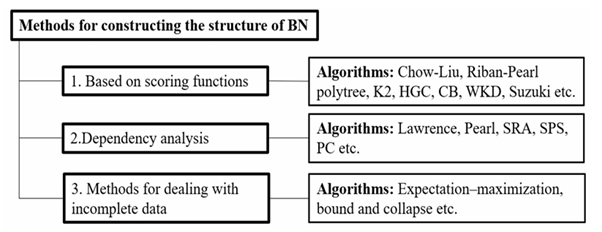
\includegraphics[width=1\linewidth]{Structure (topology) of a Bayesian network.png}
    \caption{Structure (topology) of a Bayesian network}
    \label{fig:Structure (topology) of a Bayesian network}
\end{figure}
The process of constructing the structure of a Bayesian Network (BN) can be approached using three main methods. The first method relies on scoring functions, where different candidate network structures are evaluated based on a score that balances how well the structure fits the data and its complexity, with algorithms like K2, Chow-Liu, and Hill Climbing being commonly used (Levenchuk, 2022). 

The second method is dependency analysis, which directly identifies statistical dependencies and independencies between variables using data-driven tests and then constructs the network to reflect these relationships, with algorithms such as the PC algorithm, Pearl’s method, and SRA playing key roles. 

The third method deals with incomplete data, where techniques like the Expectation-Maximization (EM) algorithm estimate both the missing data and the network structure iteratively, ensuring that incomplete observations do not compromise the learning process. These methods, whether applied individually or in combination, form the foundation for learning the causal structure that underpins a Bayesian Network.
\subsection{Structural Design:}
Finding the structure that best fits the data becomes one of the problems to solve when using BNs. Two types of machine learning perform this task: structural learning, which acquires the network structure (trees, polytrees, or multiconnected networks) from the data; and parametric learning, which has the associated conditional probabilities (table of probability) of each root node and the other variables. To determine the probability distributions linked to each vertex of the network, it is necessary to know the type of network; that is, these two learning approaches cannot be carried out independently (Muñoz-Valencia et al., 2023).
\subsection{Node Identification;} 
Creating the risk profile of each node in the Bayesian network is the first step in this process. Risk profiles are created by combining all sources of operational risk that can affect the same node and provide a basis for comparative assessment of these nodes. Mapping operational risk factors (nodes) such as internal fraud, system failures, and external events based on literature and expert input requires substantial expert knowledge. At each node, two separate tasks are performed: computation of the risk inherent to that node due only to its risks, and compounding it with the risk exposure of all incoming flows into that node. The compounded risk exposure also contributes to the mitigation efforts at that node to lower the risk exposure. This compounded risk exposure is then associated with the outgoing flow from that node. 
\subsection{Dependency Mapping:}
Establishing parent-child relationships between nodes using causal analysis. Dependency mapping and graph construction are critical steps in building a Bayesian Network. This involves identifying and establishing parent-child relationships between nodes based on causal analysis, as highlighted in Chapter 2. This step focuses on understanding how different key risk factors influence each other, determining which factors act as "parent" nodes (causal drivers) and which are "child" nodes (effects or outcomes). These relationships can be derived through expert judgment, historical data, or a combination of both, ensuring that the network accurately reflects the real-world risk profiles in financial institutions. 
\subsection{Graph Construction:} 
Creating a directed acyclic graph (DAG) that represents the identified dependencies.  The DAG visually represents the structure of the Bayesian Network, with nodes corresponding to risk factors and directed edges indicating causal dependencies between them. The acyclic nature of the graph ensures that there are no feedback loops, preserving the logical flow of cause-and-effect relationships. This graphical representation serves as the foundation for probabilistic quantification and further analysis.
\subsection{Network structure learning}
The network structure of a Bayesian Network (BN) associated with a data set can be learned using algorithms such as the grow-shrink algorithm or the hill climbing algorithm, both of which are known to produce different network structures as demonstrated by Leo, Sharma \& Maddulety (2020). The grow-shrink algorithm identifies each variable's Markov Blanket through an iterative process of adding and removing nodes based on conditional independence tests. The hill-climbing algorithm starts with an initial structure and iteratively modifies it (adding, removing, or reversing edges) to maximize a scoring function. 

Although automated structure learning is common and efficient in many fields, certain domains require the incorporation of expert knowledge, where the structure is manually defined to better reflect domain-specific causal relationships. This manual approach ensures the network aligns with expert understanding, especially in contexts like risk management or healthcare. Once the structure is learned or defined, visual examination of the resulting graph can provide valuable insights into the network’s properties and dependencies. 
\section{Quantification of Probabilities}
\subsection{Conditional Probability Tables (CPTs): }
For each node, CPTs are constructed to represent the likelihood of various outcomes based on parent node states (Sanford and Moosa, 2012). It is essential to assign probability distributions to the nodes and specify their parameters. These values should accurately represent both marginal and conditional probabilities relevant to the specific context. Such distributions can be established through experimental findings within the field, analysis of observed events, historical data, or insights provided by subject matter experts. 

\subsection{Probability Elicitation: }
Combining expert judgment with statistical techniques to estimate probabilities where data is scarce. Such probabilistic judgments are often used to provide information that cannot be obtained directly from data, observation, or first principles \parencite{Hora2017}. Probability elicitation is the most challenging part of constructing BN models, especially when there is limited availability of data like cybersecurity and when it relies on expert knowledge.  Therefore, we need to elicit probability for every possible combination of parent variables to complete the CPT of a child variable from experts, \parencite{chockalingam_probability_2023}. Using loss data and expert opinions, the Bayesian methodology can estimate operational risk loss distributions. The elicitation process of expert opinion allows a better understanding and sharing of operational risk.
\section{Data Analysis}
Cleaning and preparing an Operational risk dataset is often a mammoth task due to inconsistencies across industries, and companies. The nature of the data for modeling operational risk is the incurred losses by risk type gathered from historical data and expert elicitation as discussed earlier. Since the external and internal data may come in different formats, data transformation is necessary before the analysis. Data transformation and filtering is a mandatory step and the filtered data can then be grouped based on the classes of key risks defined. Inference in the Bayesian Network is performed to analyze the impact of different risk scenarios. Once the network has been built, we predict the probability of outcomes given initial conditions, the results should be diagnosed to estimate the most likely causes for observed outcomes.
\section{Model Validation}
Various methods were used to check and confirm the model's accuracy. Verification of the BN ensures the model functions as expected and involves manually reviewing simulation results for specific parts of the model. Adjusting parameters, like the frequency or severity of disruptions, and observing the expected outcomes also helped verify the model. Risk management professionals review the model structure and outputs to ensure alignment with real-world operational risk dynamics. After fitting the model, performance metrics were evaluated to assess how well the model's predictions align with real-world data. This involves comparing the predicted risk levels to actual loss outcomes and checking whether the predicted probabilities match the observed frequency of events. These steps help ensure the model is accurate and reliable for practical use.
\section{Scenario Analysis }
According to \textcite{Amin2016}, who asserts that each operational risk can vary in intensity or severity and has a broad range of financial effects on a company from different scenarios. Each risk event is more likely to happen under different situations, which we should consider when assessing the strength of the BN framework. Firstly, we developed discrete risk scenarios for each key risk. Each risk scenario describes a risk event, the likelihood of its occurrence, and the financial impact it has on the company. Sensitivity analysis was conducted by varying probabilities and observing changes in risk predictions. Simulations were run to evaluate the effect of hypothetical scenarios, such as cyberattacks or system failures, on operational risk.
\section{Ethical Considerations}
The study adheres to strict ethical standards in data collection and analysis, prioritizing confidentiality by maintaining the anonymity of participating experts and institutions. It ensures data integrity by relying on credible sources and verifying data accuracy. Additionally, informed consent is obtained from all participants involved in data elicitation from experts, ensuring their voluntary and informed participation.
\section{Limitations of the Methodology}
There are several challenges associated with using historical data and simulations for operational risk quantification. 
Historical data on operational failures within a company are often scarce or unavailable, especially for low-frequency, high-impact events. External loss data, while potentially useful, is difficult to apply directly due to variations in company size, risk culture, controls, and processes. Scaling external data to reflect the company’s current risk profile is complex and requires careful adjustments. 

Relying on historical data assumes that the past is a reliable predictor of the future. This can lead to the underrepresentation of unprecedented events and the overrepresentation of frequently occurring events that may have already been mitigated. The absence of data from collapsed companies introduces survival bias, and the limited data available makes it difficult to produce a good statistical BN model.

While valuable for quantitatively assessing risks, simulations also face limitations. They require detailed information about the statistical distributions and interdependencies of risks. In the absence of such information, the validity of the simulation results becomes questionable, as highlighted by the principle of "garbage in, garbage out." Moreover, risks can occur under a wide range of scenarios, and the intensity and severity of a given risk vary significantly across these scenarios. This variability adds further complexity to the modeling process.

Methods that rely on single correlation assumptions fail to capture the interdependencies between different risk scenarios and overlook the tendency of extreme events to co-occur across multiple risks. This lack of granularity in modeling correlations can lead to underestimating the compounding impact of concurrent extreme events, which are often critical in understanding operational risk. 
 
 \subsection{Tools and Software }
\begin{itemize}
    \item Python
    \item Excel
    \item Bayes Server Apk
    \item pgmpy, bnlearn
\end{itemize}
\section{Chapter Summary}
This chapter outlines the methodology used to construct, quantify, and validate a Bayesian Network (BN) framework for operational risk assessment. A mixed-methods approach integrates qualitative and quantitative techniques, leveraging historical data and expert elicitation to build a robust model.  

The model construction process begins with identifying key operational risk factors and mapping causal relationships using a Directed Acyclic Graph (DAG). Conditional Probability Distributions (CPDs) were defined through quantitative learning, combining statistical inference with expert judgment to estimate dependencies within the network. 

To quantify probabilities, empirical loss data and expert assessments were used to determine risk exposure, accounting for limited historical data. Scenario analysis and Monte Carlo simulations were run to assess the impact of various risk events, while sensitivity analysis ensures the model's robustness by examining how changes in probabilities affect outcomes. Model validation was conducted through back-testing, expert reviews, and performance metrics to ensure predictive reliability. Ethical considerations, including data confidentiality and informed consent, were upheld throughout the study.  

Despite its strengths, the methodology faces limitations, such as data scarcity, survival bias, and challenges in modeling interdependent risks. Nonetheless, the Bayesian approach provides a dynamic, data-driven framework for quantifying operational risk and supporting financial institutions in risk mitigation strategies.
